% Emacs settings: -*-mode: latex; TeX-master: "manual.tex"; -*-

\section{Advanced optical components: mirrors and guides}

This section describes advanced neutron optical
components such as supermirrors and guides.
The first subsection, however, contains 
only a description of the reflectivity of a supermirror.

\subsection{Mirror reflectivity}
\label{s:mirrorreflect}
To compute the reflectivity of the supermirrors, we use an empirical
formula derived from experimental data (see figure~\ref{f:reflectivity}). 
The reflectivity is given by the following formula
\begin{equation}
  R = \left\{
    \begin{array}{ll}
      R_0 & \textrm{if $Q \leq Q_{\rm c}$} \\
      \frac{1}{2}R_0(1 - \tanh[(Q - m Q_{\rm c})/W])(1-\alpha(Q-Q_{\rm c}))
         & \textrm{if $Q > Q_{\rm c}$}
    \end{array}
  \right.
\end{equation}

\begin{figure}
  \begin{center}
    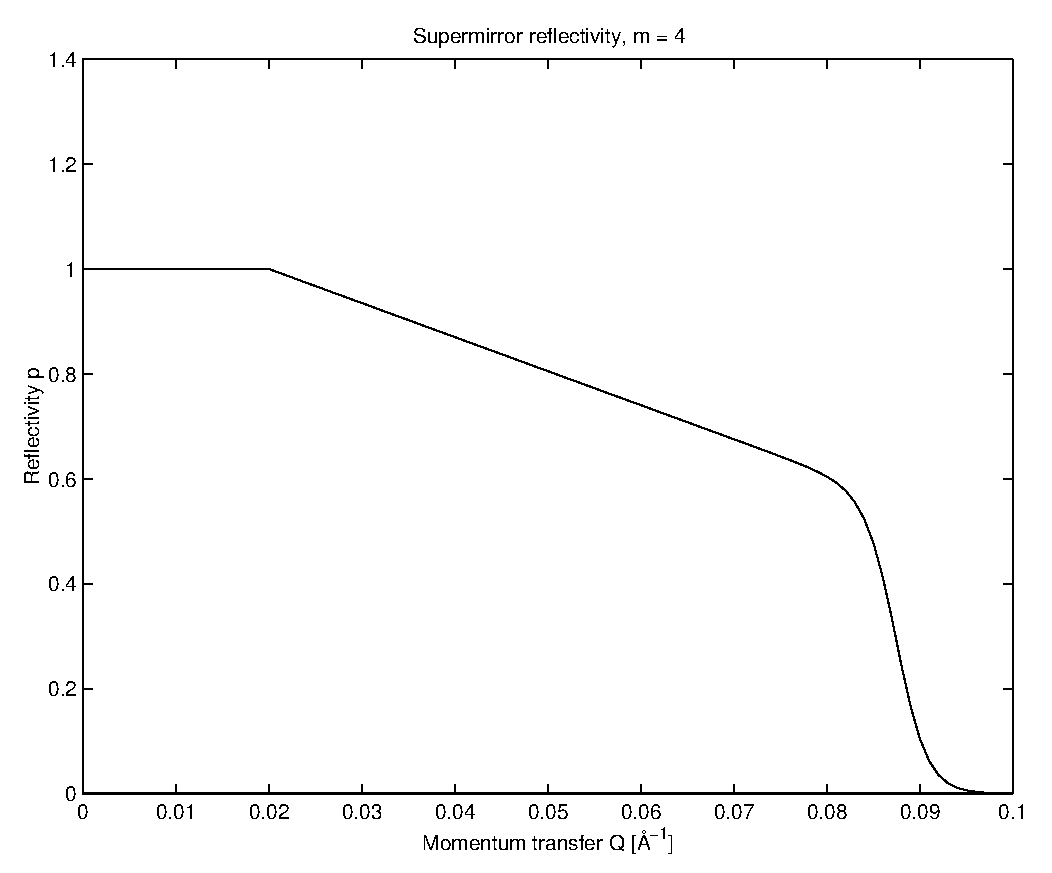
\includegraphics[width=0.6\textwidth]{figures/supermirror.eps}
  \end{center}
\caption{A typical reflectivity curve for a supermirror,
Eq.~(\protect\ref{e:reflectivity}).}
\label{f:reflectivity}
\end{figure}
Here $Q$ is the length of the scattering vector (in \AA$^{-1}$)
defined by
\begin{equation} \label{e:reflectivity}
Q = |{\bf k}_{\bf i} - {\bf k}_{\bf f}| 
  = \frac{m_{\rm n}}{\hbar} |{\bf v}_{\bf i} - {\bf v}_{\bf f}|, 
\end{equation}
$m_{\rm n}$ being the neutron mass. 
The value $m$ is a parameter determined by the mirror materials,
the bilayer sequence, and the number of bilayers.
As can be seen, $R=R_0$ for $Q < Q_{\rm c}$, which is the
critical scattering wave vector for a single layer of the mirror
material. At higher values of $Q$, the reflectivity starts falling
linearly with a slope $\alpha$ until a cut-off at $Q = m Q_{\rm c}$. 
The width of the cut-off is denoted $W$. For the curve in
figure~\ref{f:reflectivity}, the values are
$$ m=4 \qquad R_0=1 \qquad Q_{\rm c} = 0.02\mbox{ \AA}^{-1} \qquad
   \alpha = 6.49\mbox{ \AA} \qquad W=1/300\mbox{ \AA}^{-1} $$
As a special case, if $m=0$ then the reflectivity is zero for all $Q$,
   \textit{ie.} the surface is completely absorbing.

In the components, the neutron weight is adjusted with the amount $\pi_i = R$. 
To avoid spending large amounts of computation time on very low-weight
neutrons, neutrons for which the reflectivity is lower than about
$10^{-10}$ are ABSORB'ed.

\subsection{Mirror: The single mirror}

The component {\bf Mirror} 
models a single rectangular neutron mirror plate. It can
be used to \textit{e.g.}~assemble a complete neutron guide by putting multiple
mirror components at appropriate locations and orientations in the
instrument definition, much like a real guide is build from individual
mirrors.

The mirror is assumed to lie in the first quadrant of the
$x$-$y$ plane, with one corner at $(0,0,0)$. 
If the neutron trajectory intersects the mirror plate, it is
reflected, otherwise it is left untouched. Since the mirror lies in the
$x$-$y$ plane, an incoming neutron with velocity 
${\bf v}_{\rm i} = (v_x,v_y,v_z)$
is reflected with velocity ${\bf v}_{\rm f} = (v_x,v_y,-v_z)$. 
The computation of the reflectivity is handled as detailed in
section~\ref{s:mirrorreflect}.

The input parameters of this component are
the rectangular mirror dimensions $(l, h)$
and the values of $R_0, m, Q_c, W$, and $\alpha$ for the mirror.


\subsection{Guide: The guide section}

The component {\bf Guide} 
models a guide tube consisting of four flat mirrors. The
guide is centered on the $z$ axis with rectangular entrance and exit
openings parallel to the $x$-$y$ plane. The entrance has the dimensions
$(w_1,h_1)$ and placed at $z=0$. The exit is of dimensions $(w_2,h_2)$
and is placed at $z=l$ where $l$ is the guide length. See
figure~\ref{f:guide}. Neutrons not clearing the guide entrance are
ABSORB'ed. For a more general guide simulation, see the Channeled\_guide
component in section~\ref{s:channeled_guide}.

\begin{figure}
  \begin{center}
    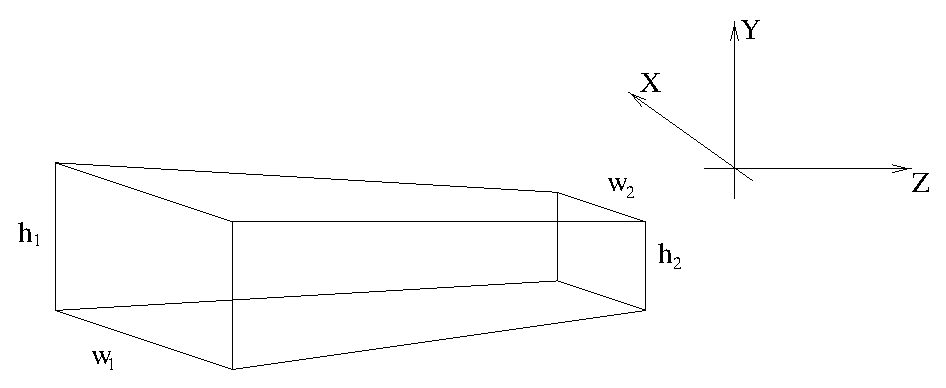
\includegraphics[width=0.9\textwidth]{figures/guide1.eps}
  \end{center}
\caption{The geometry used for the guide component.}
\label{f:guide}
\end{figure}

For computations on the guide geometry, we define the planes of the four
guide sides by giving their normal vectors (pointing into the guide)
and a point lying in the plane:
$$
\begin{array}{rclcrcl}
{\bf n}^v_1 &=& (l, 0, {(w_2 - w_1) / 2})
     & & {\bf O}^v_1 &=& (- w_1 / 2, 0, 0) \\
{\bf n}^v_2 &=& (-l, 0, {(w_2 - w_1) / 2})
     & & {\bf O}^v_2 &=& (w_1 / 2, 0, 0) \\
{\bf n}^h_1 &=& (0, l, {(h_2 - h_1) / 2})
     & & {\bf O}^h_1 &=& (0, - h_1 / 2, 0) \\
{\bf n}^h_2 &=& (0, -l, {(h_2 - h_1) / 2})
     & & {\bf O}^h_2 &=& (0, h_1 / 2, 0) \\
\end{array}
$$
In the following, we refer to an arbitrary guide side by its origin
{\bf O} and normal {\bf n}.

With these definitions, the time of intersection of the neutron with a
guide side can be computed by considering the projection onto the
normal:
\begin{equation} 
t_1 = {({\bf O} - {\bf r}_0) \cdot {\bf n} \over {\bf v} \cdot {\bf n}} 
\end{equation}
For a neutron that leaves the guide through the guide exit we have
\begin{equation}
t_2 = {l - z_0 \over v_z} 
\end{equation}
To compute the interaction of the neutron
with the guide, the neutron is initially propagated to the $z = 0$ plane of the
guide entrance. If it misses the entrance, it is ABSORB'ed. Otherwise,
we repeatedly compute the time of intersection with the
four mirror sides and the guide exit. The smallest positive $t$ thus
found gives the time of the next intersection with the guide (or in the
case of the guide exit, the time when the neutron leaves the guide). The
neutron is propagated to this point, the reflection from the side is
computed and the process is repeated until the neutron leaves the guide.

The reflected velocity ${\bf v}_{\rm f}$ of the neutron with incoming velocity
${\bf v}_{\rm i}$ is computed by the formula
\begin{equation}
 {\bf v}_{\rm f} = 
  {\bf v}_{\rm i} 
   - 2{{\bf n} \cdot {\bf v}_{\rm i} \over {|{\bf n}|^2}} {\bf n}
\end{equation}
This expression is arrived at by again considering the projection onto
the mirror normal (see figure~\ref{f:guidereflect}). The reflectivity of the
mirror is taken into account as explained in section~\ref{s:mirrorreflect}.

\begin{figure}
  \begin{center}
    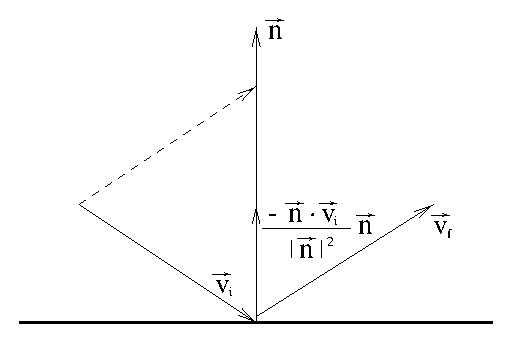
\includegraphics[width=0.5\textwidth]{figures/guide2.eps}
  \end{center}
\caption{Neutron reflecting from mirror. ${\bf v}_{\rm i}$ and 
${\bf v}_{\rm f}$ are the initial and final velocities, respectively,
and {\bf n} is a vector normal to the mirror surface.}
\label{f:guidereflect}
\end{figure}

There are a few optimizations possible here to avoid redundant
computations. Since the neutron is always inside the guide during the
computations, we always have 
$({\bf O} - {\bf r}_0) \cdot {\bf n} \leq 0$. 
Thus $t \leq 0$ if ${\bf v} \cdot {\bf n} \geq 0$, so in this case
there is no need to actually compute $t$. Some redundant computations
are also avoided by utilizing symmetry and the fact that many
components of {\bf n} and {\bf O} are zero.

The input parameters of this component are
the opening sizes of the entry and exit point of the
guide, $(w_1, h_1)$ and $(w_2, h_2)$, respectively,
the guide length, $l$,
and the values of $R_0, m, Q_c, W$, and $\alpha$ for the mirror.


\subsection{Channeled\_guide: A guide section component with multiple channels}
\label{s:channeled_guide}

The component Channeled\_guide is a more flexible variation of the Guide
component described in the previous section. It allows the specification
of different supermirror parameters for the horizontal and vertical
mirrors, and also implements guides with multiple channels as used in
neutron bender devices. By setting the $m$ value of the supermirror
coatings to zero, nonreflecting walls are
simulated; this may be used to simulate a Soller collimator.

The channel walls are assumed to be infinitely absorbing. The
implementation is basen on that of the Guide component. Initially, the
channel which the neutron will enter is computed. The $x$ coordinate is
then shifted so that the channel can be simulated as a single instance
of the Guide component. Finally the coordinates are restored when the
neutron exits the guide or is absorbed.

The input parameters are \textit{w1}, \textit{h1}, \textit{w2},
\textit{h2}, and \textit{l} to set the guide dimensions in meters as for
the Guide component (entry window, exit window, and length); \textit{k}
to set the number of channels; \textit{d} to set the thickness of the
channel walls, in meters; and \textit{R0}, \textit{W}, \textit{Qcx},
\textit{Qcy}, \textit{alphax}, \textit{alphay}, \textit{mx}, and \textit{my} to
set the supermirror parameters as described above (the names with \textit{x}
denote the vertical mirrors, and those with \textit{y} denote the horizontal
ones).
